\subsection{}
There comes 5 assumptions with monopolistic competition,
it is a hybrid of monopoly and perfect competition.
\begin{enumerate}
    \item Price makers.
    \item Many buyers and many sellers (still not as many as perfect competition).
    \item The product is heterogeneous (differentiated).
    \item No barriers to entry or exit.
    \item Imperfect information.
\end{enumerate}
Examples of monopolistic competition are fast food restaurants, clothing stores and gas stations.
Advertising exists because of the differentiation of products.
\par
Demand is downward sloping but more elastic than a monopoly.\\
The demand curve is equal to average revenue.\\
The marginal revenue curve is twice as steep as the demand curve.\\
The shut-down point exists but is not important to know it's location.\\
Marginal cost intersects the minimum of the average cost curve.
\begin{figure}[H]
    \centering
    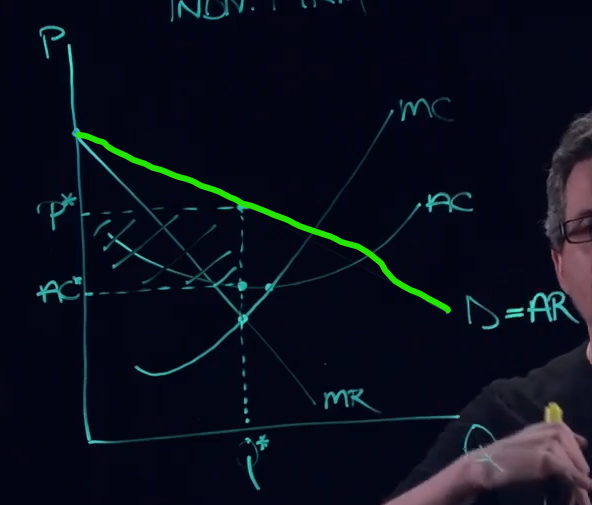
\includegraphics[width=0.5\textwidth]{Chapter11/MonopolisticCompetition.png}
    \caption{Monopolistic Competition}
    \label{fig:monopolisticcompetition}
\end{figure}
If a firm is making a profit in monopolistic competition, other firms will enter the market.\\
If a firm is making a loss in monopolistic competition, the firm will exit the market.\\
All firms in the long run will break even.
\par
A monopolistic competition has a trade off with perfect competition.
In exchange for operating below optimal efficiency, the consumer has to pay a premium for having choice between
differentiated products. If firms increased production, they would give up the differentiation.\\
The concept of firms in a monopolistic competition operating below optimal efficiency is called excess capacity.